\section{A MAC Layer in Mote Runner}
\begin{frame}[fragile]
  \frametitle{Design strategy}
  \begin{itemize}
    \item Mac class behaviours:
    \begin{itemize}
      \item Coordinator -> Beacon enabled, Slotted CSMA/CA
      \item Unassociated -> Handles association with a Coordinator
      \item Associated -> Sends data from upper layer and receives data from Coordinator
    \end{itemize}
    \item Flexibility:
    \begin{itemize}
    	\item State changes are ruled by Mac class through events
    	\item Mac can handle more than one state -> Mac - entities
    	\begin{itemize}
	  \item e.g.: Coordinator - Associated
    	\end{itemize}

    \end{itemize}
  \end{itemize}
\end{frame}

\begin{frame}[fragile]
  \frametitle{Timing with beacon}
  \begin{itemize}
    \item It grants synchronization between mote and coordinator
    \item Realized with a timer and scheduled events
  \end{itemize}
  \begin{figure}
    \centering
    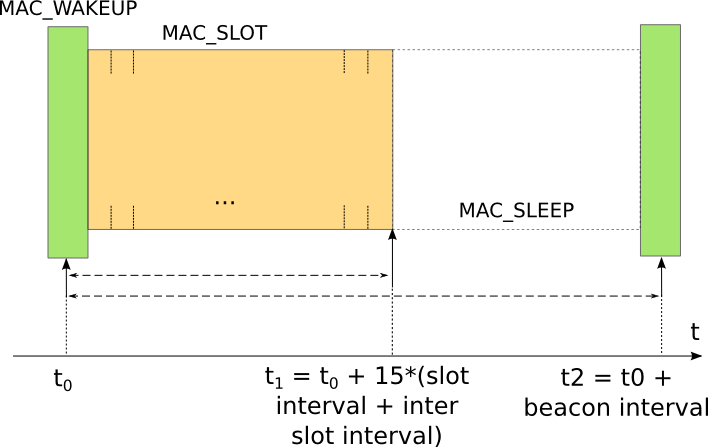
\includegraphics[width=.7\textwidth]{img/MAC_STATES.png}
  \end{figure}
\end{frame}

\begin{frame}[fragile]
  \frametitle{Mac Coordinator Behaviour}
  \vspace{-2.7em}
  \begin{figure}
    \centering
    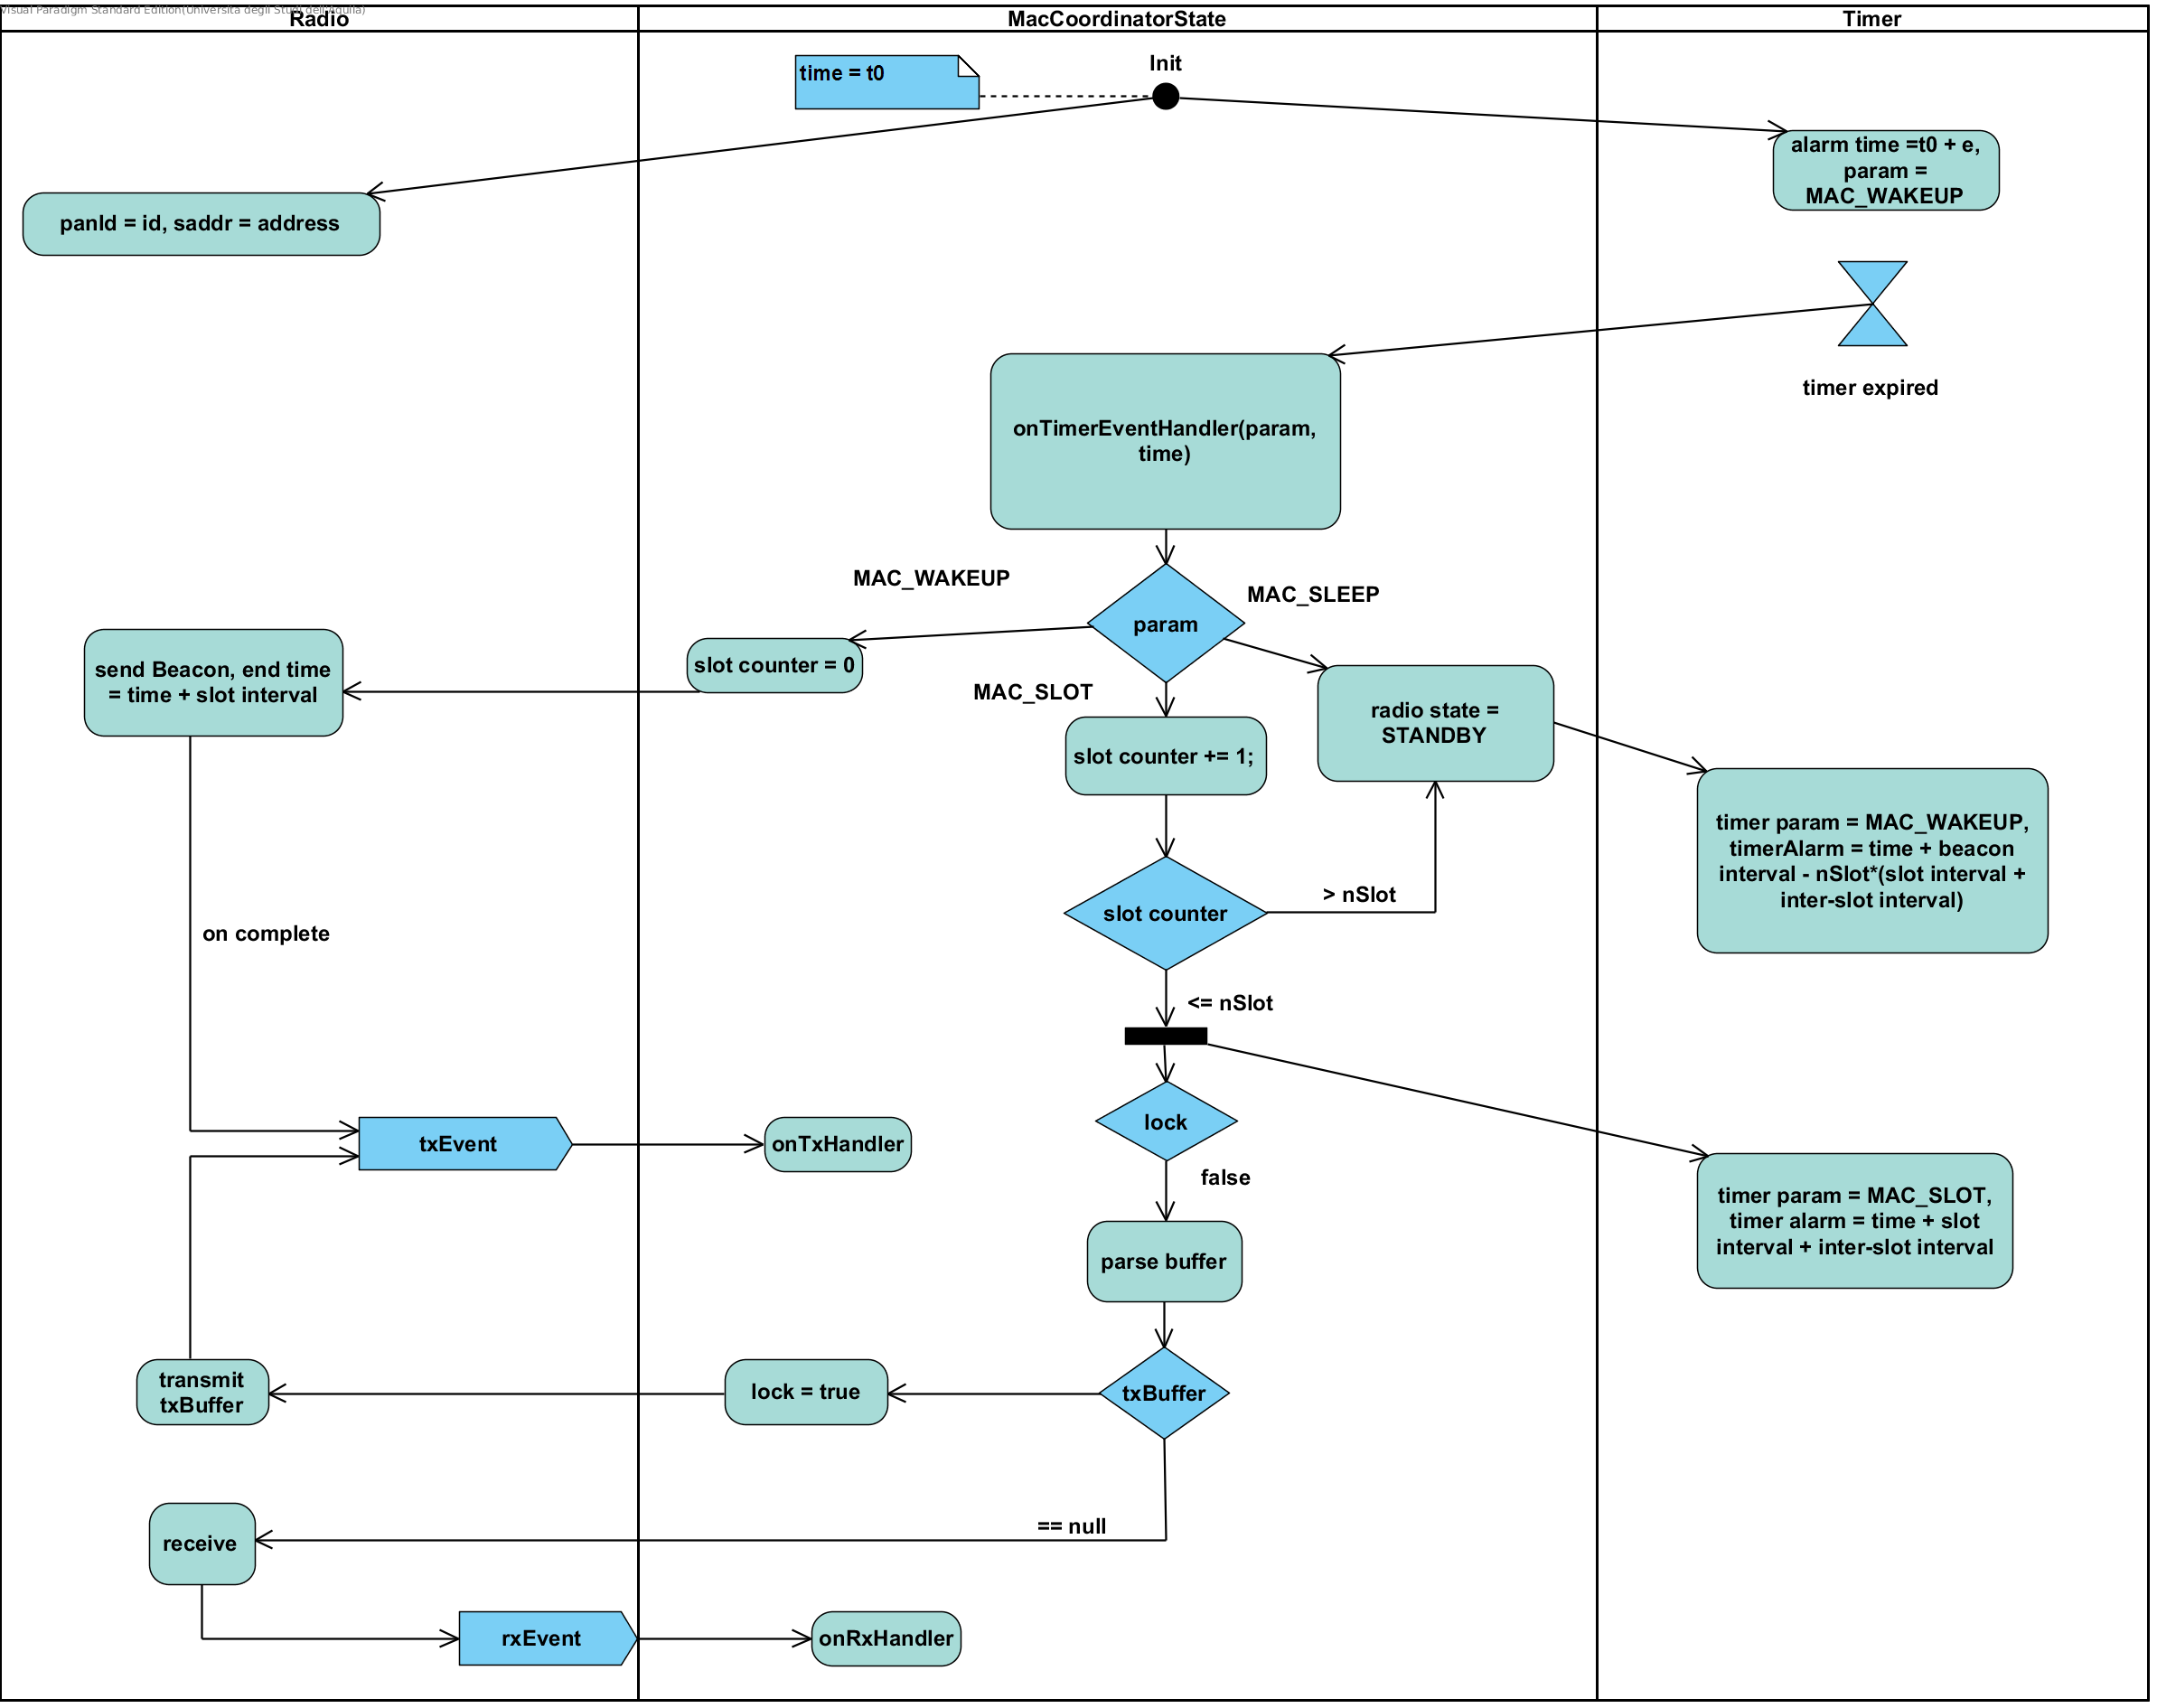
\includegraphics[width=.99\textwidth]{img/MAC_COORDINATOR.png}
  \end{figure}
\end{frame}

\begin{frame}[fragile]
  \frametitle{Example}
  \vspace{-2em}
  The node associates with coordinator, then responds to beacon pending list and gets data.
  \begin{figure}
    \centering
    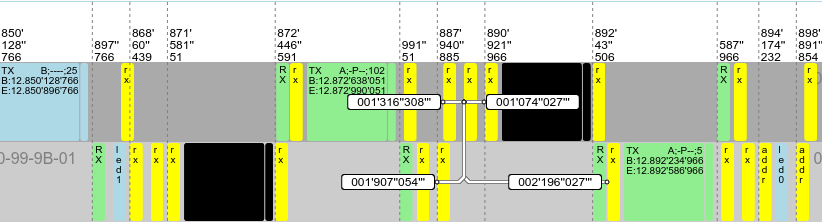
\includegraphics[width=\textwidth]{img/associazione.png}
  \end{figure}
  \begin{figure}
    \centering
    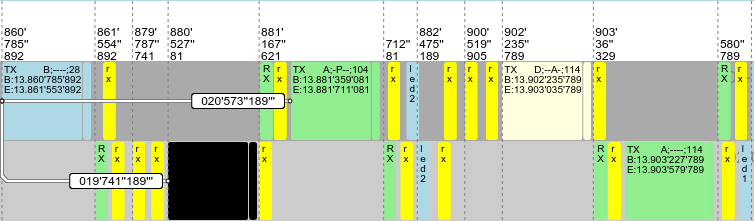
\includegraphics[width=\textwidth]{img/dataIndirect.png}
  \end{figure}
\end{frame}


